\section{Бутстреп-пары против бутстреп-остатков}

Читатель, возможно, заметил интересный факт, теперь у нас есть два различных способа построения бутстреп регрессионной модели. Метод, описанный в главе 7, выбирает пары $\textbf{x}_i = (\textbf{c}_i, y_i)$, так что бутстреп набор данных $\textbf{x}^*$ имел форму
\begin{equation}
	\textbf{x}^* = \{ (\textbf{c}_{{i}_1}, y_{{i}_1}), (\textbf{c}_{{i}_2}, y_{{i}_2}), \ldots, (\textbf{c}_{{i}_n}, y_{{i}_n}) \},
\end{equation}
для $i_1, i_2, \ldots, i_n$ в случайной выборке целых чисел от $1$ до $n$. Обсуждаемый в этой главе метод (9.24), (9.25), (9.26) можно назвать «бутстрепом остатков». Он создает бутстреп наборы данных в форме
\begin{equation}
	\textbf{x}^* = \{ (\textbf{c}_1, \textbf{c}_1 \hat{\bm{\beta}} + \hat{\varepsilon}_{{i}_1}), (\textbf{c}_2, \textbf{c}_2 \hat{\bm{\beta}} + \hat{\varepsilon}_{{i}_2}), \ldots, (\textbf{c}_n, \textbf{c}_n \hat{\bm{\beta}} + \hat{\varepsilon}_{{i}_n}) \}.
\end{equation}

\noindent
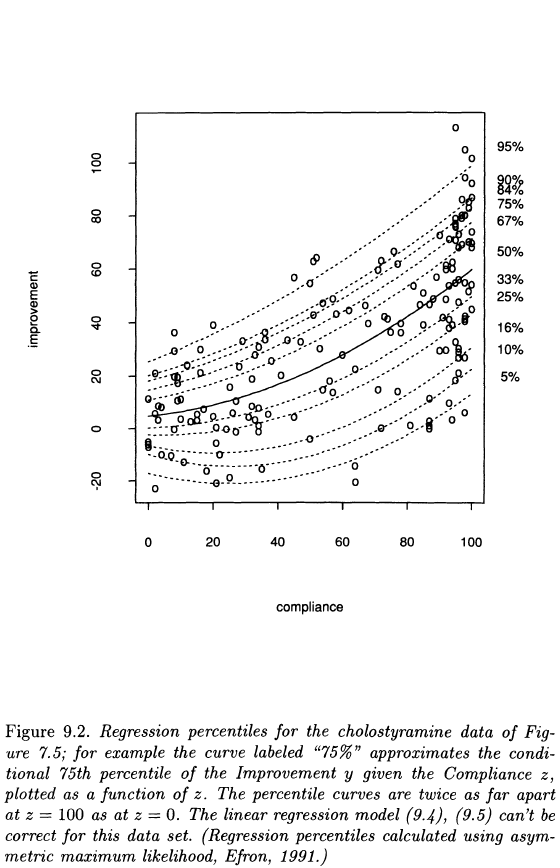
\includegraphics[width=\linewidth]{9/f92}
\newline

Какой бутстреп метод лучше? Ответ зависит от того, насколько мы доверяем модели линейной регрессии (9.4). Эта модель говорит, что разность между $y_i$ и его средним значением $\mu_i = \textbf{c}_i \bm{\beta}$ не зависит от $\textbf{c}_i$; он имеет одинаковое распределение «$F$» независимо от $\textbf{c}_i$. Это --- сильное предположение, которое может оказаться неверным, даже если модель математического ожидания $\mu_i = \textbf{c}_i \bm{\beta}$ верна. Это не соответствует данным про холостирамин на рис. 7.4.

На рисунке 9.2 показаны \textit{процентили регрессии} для данных про холостирамин. Например, кривая, обозначенная «$75$\%», аппроксимирует условный $75$-й процентиль показателя улучшения $y$ как функцию показателя соответствия $z$. Вблизи любого заданного значения $z$ около $75$\% нанесенных на график точек лежат ниже кривой. Модель (9.4), (9.5) предсказывает, что эти кривые будут находиться на одинаковом расстоянии друг от друга для всех значений $z$. Вместо этого кривые расходятся по мере увеличения $z$, находясь вдвое дальше друг от друга при $z = 100$, чем при $z = 0$. Другими словами, ошибки $\varepsilon_i$ в (9.4) стремятся быть вдвое больше при $z = 100$, чем при $z = 0$.

Бутстреп-пары менее чувствительны к предположениям, чем бутстреп-остатки. Стандартная оценка ошибки, полученная с помощью бутстреп-пар (9.31), дает разумные результаты, даже если (9.4), (9.5) полностью неверны. Единственное предположение, стоящее за (9.31), состоит в том, что исходные пары $\textbf{x}_i = (\textbf{c}_i, y_i)$ были случайным образом выбраны из некоторого распределения $F$, где $F$ --- распределение на $(p+1)$-мерных векторах $(\textbf{c}, y)$. Даже если (9.4), (9.5) верны, нет ничего плохого в бустреп-парах, как показано в (9.31); можно показать, что ответ (9.31) приближается к ответу (9.32) по мере увеличения числа пар $n$. Простая модель для данных о гормонах (9.12) была повторно проанализирована методом бутстреп-пар. $B = 800$ бутстреп-репликаций дали
\begin{equation}
	\hat{\text{se}}_{800} (\hat{\beta}_0) = 0.77 \quad \hat{\text{se}}_{800}(\hat{\beta}_1) = 0.0045,
\end{equation}
что не сильно отличается от результатов в таблице 9.2.

Можно привести и обратный аргумент. Модель (9.4), (9.5) не обязательно должна выполняться идеально, чтобы бутстреп остатков, как в (9.32), давал разумные результаты. Более того, различия в распределении ошибок, как и в данных о холостирамине, могут быть включены в модель (9.4), (9.5), что приведет к более подходящей версии бутстреп-остатков; см. модель (9.42). Возможно, наиболее важным моментом здесь является то, что бутстреп не является однозначно определенной концепцией. Рисунок 8.3 может быть реализован по-разному для одной и той же задачи, в зависимости от того, как интерпретируется вероятностная модель $P \to \textbf{x}$.

Когда мы осуществляем бустреп остатков, бутстреп наборы данных $\textbf{x}^* = \{(\textbf{c}_1, y_1^*), (\textbf{c}_2, y_2^*), \ldots, (\textbf{c}_n, y_n^*)\}$ имеют векторы признаков $\textbf{c}_1, \textbf{c}_2, \ldots, \textbf{c}_n$ в точности такие же, как и для фактического набора данных $\textbf{x}$. Это кажется неестественным для данных о гормонах, где $\textbf{c}_i$ включает $z_i$, затраченное количество часов, которое является такой же случайной величиной, как и переменная ответа $y_i$, оставшееся количество гормона.

Даже когда признаки генерируются случайным образом, есть причины проводить анализ так, как если бы они были фиксированными. Коэффициенты регрессии имеют большую стандартную ошибку, когда признаки имеют меньшее стандартное отклонение. Рассматривая признаки как фиксированные константы, мы получаем стандартную ошибку, которая отражает точность, связанную с выборкой фактически наблюдаемых признаков. Однако, как показывает (9.33), разница между $\textbf{c}_i$ фиксированной и $\textbf{c}_i$ случайной обычно не сильно влияет на оценку стандартной ошибки.